\chapter{Usabilidade}

Neste capítulo abordaremos os conceitos de usabilidade e suas relações, além de entender a sua importância em um software, apresentar os modelos de ciclo de vida utilizados na usabilidade e mostrar como pode ser inserida a usabilidade no ciclo de desenvolvimento empírico de software.

\section{Conceitos de Usabilidade}

A usabilidade é um termo que começou a ser utilizado pela Ciência Cognitiva e depois pela Psicologia e Ergonomia em substituição ao termo ``amigável'' ~\cite{dias2006}.
%TODO: aspas as em latex é assim: `` '' 
% 
A usabilidade é um conjunto de propriedades de uma interface que reúne os seguintes componentes: fácil aprendizado, eficiência, capacidade de memorização, baixo índice de erros, satisfação e prazer ao uso~\cite{nielsen1994}.
%
Ainda de acordo com \citeonline{nielsen2007} usabilidade é um atributo de qualidade relacionado à facilidade de uso de algo. Refere-se a rapidez com que os usuários podem aprender a usar alguma coisa, a eficiência deles ao usá-la, o quanto lembram daquilo, seu grau de propensão a erros e o quanto gostam de utilizá-la. 
%
\begin{comment}
Ainda, usabilidade é definida como o fator que assegura que um produto ou serviço é fácil de usar, eficiente e agradável a partir do ponto de vista do usuário~\cite{preece2007}.
%TODO: Um parágrafo apresenta uma ideia completa: com início, meio e fim.
% eu juntei os trechos acima em %um único parágrafo.


A qualidade em uso engloba o contexto do ambiente de trabalho para caracterizar a satisfação de uso, focando não apenas no usuário, mas em seu comportamento ao interagir com um sistema computacional.
%
O conceito de qualidade em uso mais difundido é o de usabilidade que engloba a facilidade e a eficiência de aprendizado de uso, bem como a satisfação do usuário.
%
Esse conceito de qualidade em uso é defendido pela norma ~\citeonline{ISO:9126}, que define usabilidade como  capacidade do produto de software ser compreendido, aprendido, operado e atraente ao usuário, quando usado sob condições específicas.
%
Já a norma ~\citeonline{iso:9241} define usabilidade como a capacidade de um produto ser usado por usuários específicos para alcançar objetivos específicos com eficácia, eficiência e satisfação em um contexto de uso específico. Essa norma define alguns termos que são amplamente utilizados quando trata-se de usabilidade.
\end{comment}

 A norma ~\citeonline{iso:9241} define alguns termos que são amplamente utilizados quando trata-se de usabilidade:

\begin{itemize}
\item \textbf{Eficácia:} é a capacidade que os sistemas conferem a diferentes tipos de usuários para alcançar seus objetivos em número e com a qualidade necessária. 

\item \textbf{Eficiência:} é a quantidade de recursos que os sistemas solicitam aos usuários para a observação de seu objetivos com o sistema.

\item \textbf{Satisfação:} é a emoção que os sistemas proporciona, aos usuários em face dos resultados obtidos e dos recursos necessários para alcançar tais objetivos. 

\item \textbf{Tarefa:} Objetivo a ser atingido ou um resultado a obter.

\item \textbf{Usuários:} Pessoas que utilizam alguma instância do sistema.

\item \textbf{Contexto:} Conjunto de elementos, onde se destacam: o ambiente físico, a tecnologia utilizada e a a motivação.
\end{itemize}

Adicionalmente, existem metas de usabilidade que servem para guiar o desenvolvimento de um software~\cite{preece2007}. São elas:

\begin{enumerate}
	\item \textbf{Utilidade:} é a medida na qual o sistema propicia o tipo certo de funcionalidade, de maneira que os usuários possam realizar aquilo de que precisam ou desejam.
	\item \textbf{Eficácia:} refere-se ao quanto um sistema é bom em fazer o que se espera dele.
	\item \textbf{Eficiência:} refere-se à maneira como o sistema auxilia os usuários na realização de suas tarefas.
	\item \textbf{Segurança:} implica em proteger o usuário de condições perigosas e situações indesejáveis.
	\item \textbf{Facilidade de aprendizado:} refere-se a qual fácil é aprender a usar o sistema.
	\item \textbf{Facilidade de lembrar como se usa:} refere-se à facilidade de lembrar como utiliza um sistema, depois de já ter aprendido como usar.
\end{enumerate}

Para entender como usabilidade está inserida no ciclo de vida do desenvolvimento de software, precisamos compreender as relações que o termo tem com as diversas áreas que a envolve: 

\begin{description}

\item[Interação Humano Computador:]

%
A interação humano computador \emph{Human Computer Interaction} (HCI) tem o principal objetivo de melhorar a eficácia e proporcionar satisfação do usuário, desnvolvendo sistemas computacionais nos quais os usuários possam executar tarefas com segurança, eficiência e satisfação \\ ~\cite{preece2007}.
	
\item[Arquitetura da Informação:]


A arquitetura da informação é a ciência de estruturar, bem como, de organizar os ambientes informacionais para ajudar as pessoas a encontrarem e administrarem informações~\cite{garret2003}.
%
O arquiteto de informação deve balancear as necessidades do usuário com os objetivos do negócio~\cite{rosenfeld1998}.

\item[Ergonomia:]
%
A ergonomia pois visa proporcionar eficácia e eficiência para o usuário através da adaptação do trabalho ao homem.
%
O seu objetivo é garantir que sistemas e dispositivos estejam adaptados às maneiras de pensar, agir e trabalhar do usuário~\cite{cybis2010} .

\item[\emph{Design} Centrado no usuário:]

Para~\citeonline{norman2006design} \emph{design} centrado no usuário é uma filosofia baseada nas necessidades e interesses dos usuário, com ênfase em fazer produtos usáveis e inteligíveis. 
%
As pessoas que utilizarão um produto ou serviço sabem de suas necessidades, metas e preferências, e é papel do \emph{design} descobrir isso para projetar para eles -- essa é a filosofia por trás do \emph{design} centrado no usuário~\cite{saffer2010designing}.

\item[Design de Interação:]

O \emph{design} de interação redireciona a preocupação que se tinha apenas em produzir algo que funcionasse para produzir algo que será fácil de utilizar, agradável e eficaz na perspectiva do usuário, trazendo a usabilidade para dentro do processo de \emph{design}~\cite{preece2007}.
%
Bill Verplank resume \emph{design} de interação a partir da resposta de três perguntas sobre: como você age? como você sente? como você compreende?\cite{moggridge2006}. 
%


\item[Engenharia de Usabilidade:]

A engenharia de usabilidade ocupa-se da interface com o usuário que interliga as funções do sistema com os usuários de forma que a interface do sistema seja agradável, intuitivo, eficiente e fácil de operar ~\cite{cybis2010}. Já a engenharia de software ocupa do desenvolvimento do núcleo funcional de um sistema interativo formado por estruturas de dados, algoritmos e recursos de processamento de dados. Esse núcleo é construído de forma que o sistema funcione bem, de forma correta, rápida e sem erros.
%


\item[Experiência do Usuário - UX: ]

Toda a interação com um produto, serviço ou marca. O termo é usado frequentemente para sintetizar toda a experiência com um produto de software. Não engloba  somente as funcionalidades e sim o quanto o aplicativo é agradável ao usuário~\cite{travis2013}.
%	


\end{description}
%TODO: vamos deixar o parágrafo abaixo com um fechado desta seção

A usabilidade está relacionada com os fatores humanos e corresponde ao estudo de como usuários se relacionam com qualquer produto. A interação humano computador está baseada na usabilidade e foca no modo como as pessoas se relacionam com softwares.

%------------------------------------------------------------------------------%. 

\section{Técnicas e Métodos da Engenharia de Usabilidade}

%TODO Colocar apenas uma tabela com o nome da técnica e uma descrição sussinta. O restante vai para o apêndice.

Existem diversas técnicas e métodos que são utilizados pela interação humano computador para desenvolver um sistema com usabilidade. ~\citeonline{cybis2010} divide as técnicas da engenharia de usabilidade em três tipos: Concepção, Análise e Avaliação. 

\subsection{Métodos e Técnicas de Concepção}

Os métodos de concepção são utilizados para implementar as especificações e os requisitos para a interface e usabilidade de um sistema:

\newpage

\begin{table}[h]
\centering
\begin{tabular}{|p{4cm}|p{8cm}|}
\hline 
Técnica & Descrição \\ 
\hline 
Brainstorming & É uma técnica utilizada para obter ideias, entrar em consenso sobre problemas ou novas propostas \\ 
\hline 
Storyboard & É uma representação das interações entre os usuários e o sistema em seu ambiente de trabalho \\ 
\hline 
Card Sorting & É uma técnica usada para descobrir como o usuário classifica determinada informação em sua mente. \\ 
\hline 
Diagramas de Afinidade & São utilizadas para organizar uma grande quantidade de itens em grupos lógicos. \\ 
\hline 
Protótipos & São utilizados para esclarecer os requisitos específicos para o projeto de interface do sistema. \\ 
\hline 
\end{tabular}
\caption{Métodos e Técnicas de Concepção}
\end{table}


No apêndice \ref{apendice1} há uma definição melhor de como é aplicada cada técnica.


\subsection{Métodos e Técnicas de Análise}

Os métodos e técnicas de análise são utilizados para buscar informações sobre a usabilidade de um sistema. Podem ser feitas análises do perfil do usuário, do ambiente de uso, das tarefas, possibilidades e restrições do sistema, etc. As técnicas mencionadas na tabela ~\ref{analise-usabilidade} visam apoiar a equipe na busca de informações sobre a usabilidade de um sistema. 

\newpage

\begin{table}[h]
\begin{tabular}{|p{4cm}|p{11cm}|}
\hline 
Técnica & Descrição \\ 
\hline 
Persona & A técnica de persona descreve o perfil de uma pessoa fictícia envolvida com o produto. Trata-se de inventar um conjunto de pessoas (três ou quatro) que estejam dentro da população de usuários pretendidos e descrevê-las em detalhes. \\ 
\hline 
Entrevistas Tradicionais & Técnica utilizada para obter as opiniões tanto dos usuários atuais como dos futuros usuários dos sistemas. \\ 
\hline 
Eyetracking & É uma técnica que rastreia o movimento dos olhos e da cabeça para registrar a tomada de informações numa interface. \\ 
\hline 
Questionários de Perfil de uso & É uma técnica utilizada para obter informações sobre as características reais dos usuários de um sistema e saber como eles realmente utilizam tais ferramentas. \\ 
\hline 
Questionários de Satisfação & São questionários utilizados para medir a satisfação do usuário ao utilizar um sistema. Resultam da avaliação subjetiva pelo usuário. \\ 
\hline 
Grupo Focal & É uma reunião informal de usuários que manifestam suas opiniões sobre o determinado assunto, que pode ser tanto uma oportunidade de novas funcionalidades ou algum problema específico. \\ 
\hline 
Diários & É uma técnica na qual os usuários carregam consigo um pequeno diário para nele anotar as informações do seu dia-a-dia na utilização do sistema.\\ 
\hline 
Bechmarking de Usabilidade & É um método utilizado para criar critérios de avaliação e seleção de representantes para criar características desejáveis para o futuro sistema. \\ 
\hline 
Cenários de Uso & É uma técnica simples e eficaz para analisar e comunicar uma parte das especificações de requisitos produzidos para a usabilidade e a interface. \\ 
\hline 
Observação & Essa técnica caracteriza-se por um pesquisador observando o usuário e tomando notas, enquanto este trabalha em seu contexto usual. \\ 
\hline  
\end{tabular} 
\caption{Métodos e Técnicas de Análise da usabilidade}
\label{analise-usabilidade}
\end{table}

No apêndice \ref{apendice1} estão detalhadas as técnicas mencionadas nesta seção.

\subsection{Métodos e Técnicas de Avaliação da Usabilidade}
\label{metodos_avaliacoes}
Utilizados para avaliar a qualidade das interações entre o usuário e o sistema.
%
As avaliações de interface podem ser divididas quanto a: formas, tipo de dados e o local da avaliação. Quanto a forma, temos objetiva, quando são baseadas em técnicas que utilizam medições quantitativas em vez de opiniões dos usuários/especialistas e subjetivas, quando são baseadas em opiniões e relatos de usuários e especialistas. Já quanto ao tipo de dados podem ser definidas como: quantitativa, quando envolvem medidas e tendem a ser vistas como objetivas e imparciais, e qualitativas quando envolvem descrições e relatos e são vistas como subjetivas. Quanto ao local da avaliação podem ser feita em laboratório, onde o ambiente é controlado ou estudo de campo quando estão situadas no contexto do mundo real no qual o sistema é utilizado.


\begin{table}[h]
\centering
\begin{tabular}{|p{4cm}|p{8cm}|}
\hline 
Técnica & Descrição \\ 
\hline 
Checklists & É uma técnica de inspeção que oferece uma maneira de abordagem rápida, fácil e de baixo custo para a avaliação de uma interface. Permite com que usuários que não são especialistas em ergonomia identificarem problemas menores e repetitivos ~\cite{cybis2010}. \\ 
\hline 
Avaliação heurística & É uma técnica de avaliação realizada por especialistas de usabilidade para identificar problemas iniciais de usabilidade de um sistema. \\ 
\hline 
Percurso Cognitivo & É um método de inspeção de usabilidade que tem como objetivo avaliar a interface considerando a facilidade da interface \\ 
\hline 
Testes de usabilidade & É um dos métodos de teste de experiência do usuário (UX) mais frequentemente utilizado e conhecido entre aqueles que não são projetistas da UX. Realizar testes com usuários é o núcleo do \emph{Design} Centrado no Usuário, pois é através destes que podemos saber se as reais expectativas dos usuários são atendidas ~\cite{santos2012}. \\ 
\hline 
\end{tabular} 
\caption{Métodos e Técnicas de Avaliação}
\end{table}

De acordo com ~\citeonline{preece2007} cada método de avaliação possui características e pode ser aplicado em diferentes situações.
%
Eles diferem entre si em vários aspectos. É preciso entender as diferentes características de cada método para se definir qual deles é o mais apropriado para avaliar a interface de um software em um determinado contexto.
%
No estudo de caso aplicamos as seguintes técnicas:

\begin{description}

\item[Checklists:]

	É uma técnica de inspeção que oferece uma maneira de abordagem rápida, fácil e de baixo custo para a avaliação de uma interface. Permite com que usuários que não são especialistas em ergonomia identificarem problemas menores e repetitivos ~\cite{cybis2010}.
%
Várias vantagens são encontradas na utilização dessa técnica como: redução de custos de avaliação por não precisar de especialistas; sistematização das avaliações; reduz a subjetividade dos processos de avaliação e fornece um conhecimento ergonômico sobre o que avaliar.
%
Os checklists utilizados encontra-se na seção apêncie \ref{checklist}.

\item[Avaliação heurística:]


	Representa um julgamento de valor sobre as qualidades ergonômicas das interfaces Humano-Computador. Essa avaliação é realizada por especialistas em ergonomia e usabilidade. Eles examinam o sistema interativo e diagnosticam os problemas ou as barreiras que os usuários provavelmente encontrarão durante a interação ~\cite{cybis2010}.

	O principal objetivo desse tipo de avaliação é avaliar a interface em fases iniciais do sistema, sem o envolvimento do usuário. Os graves problemas de interface devem ser localizados antes que realizem os testes de usabilidade com usuários reais ~\cite{santos2012}.

	As avaliações mais utilizadas são as 10 heurísticas de ~\citeonline{nielsen1994}. São elas:

	\begin{itemize}
		\item{\textbf{Diálogos simples e naturais:} Deve-se apresentar exatamente a informação que o usuário precisa no momento, nem mais nem menos. A seqüência da interação e o acesso aos objetos e operações devem ser compatíveis com o modo pelo qual o usuário realiza suas tarefas.}
		\item{\textbf{Falar a linguagem do usuário:} A terminologia deve ser baseada na linguagem do usuário e não orientada ao sistema. As informações devem ser organizadas conforme o modelo mental do usuário.}
		\item{\textbf{Minimizar a sobrecarga de memória do usuário:} O sistema deve mostrar os elementos de diálogo e permitir que o usuário faça suas escolhas, sem a necessidade de lembrar um comando específico.}
		\item{\textbf{Consistência e Padrões:} Um mesmo comando ou ação deve ter sempre o mesmo efeito. A mesma operação deve ser apresentada na mesma localização e deve ser formatada/apresentada da mesma maneira para facilitar o reconhecimento.}
		\item{\textbf{Feedback:} O sistema deve informar continuamente ao usuário sobre o que ele está fazendo. 10 segundos é o limite para manter a atenção do usuário focalizada no diálogo.}
		\item{\textbf{Saídas claramente marcadas:} O usuário controla o sistema. Ele pode, a qualquer momento, abortar uma tarefa, ou desfazer uma operação e retornar ao estado anterior.}
		\item{\textbf{Atalhos:} Para usuários experientes executarem as operações mais rapidamente. Abreviações, teclas de função, duplo clique no mouse, função de volta em sistemas hipertexto. Atalhos também servem para recuperar informações que estão numa profundidade na árvore navegacional a partir da interface principal.}
		\item{\textbf{Boas mensagens de erro:} Linguagem clara e sem códigos. Devem ajudar o usuário a entender e resolver o problema. Não devem culpar ou intimidar o usuário.}
		\item{\textbf{Prevenir erros:} Evitar situações de erro. Conhecer as situações que mais provocam erros e modificar a interface para que estes erros não ocorram.}
		\item{\textbf{Ajuda e documentação:} O ideal é que um software seja tão fácil de usar (intuitivo) que não necessite de ajuda ou documentação. Se for necessária a ajuda deve estar facilmente acessível e on-line.}
	\end{itemize}


	As avaliações podem ser feitas em planilhas (como a figura \ref{planilha}), onde são descritos o local do problema de usabilidade, sua descrição, a heurística que foi desobedecida e a criticidade do problema (alta, média ou baixa).

	\begin{figure}[h]
    	\centering
    	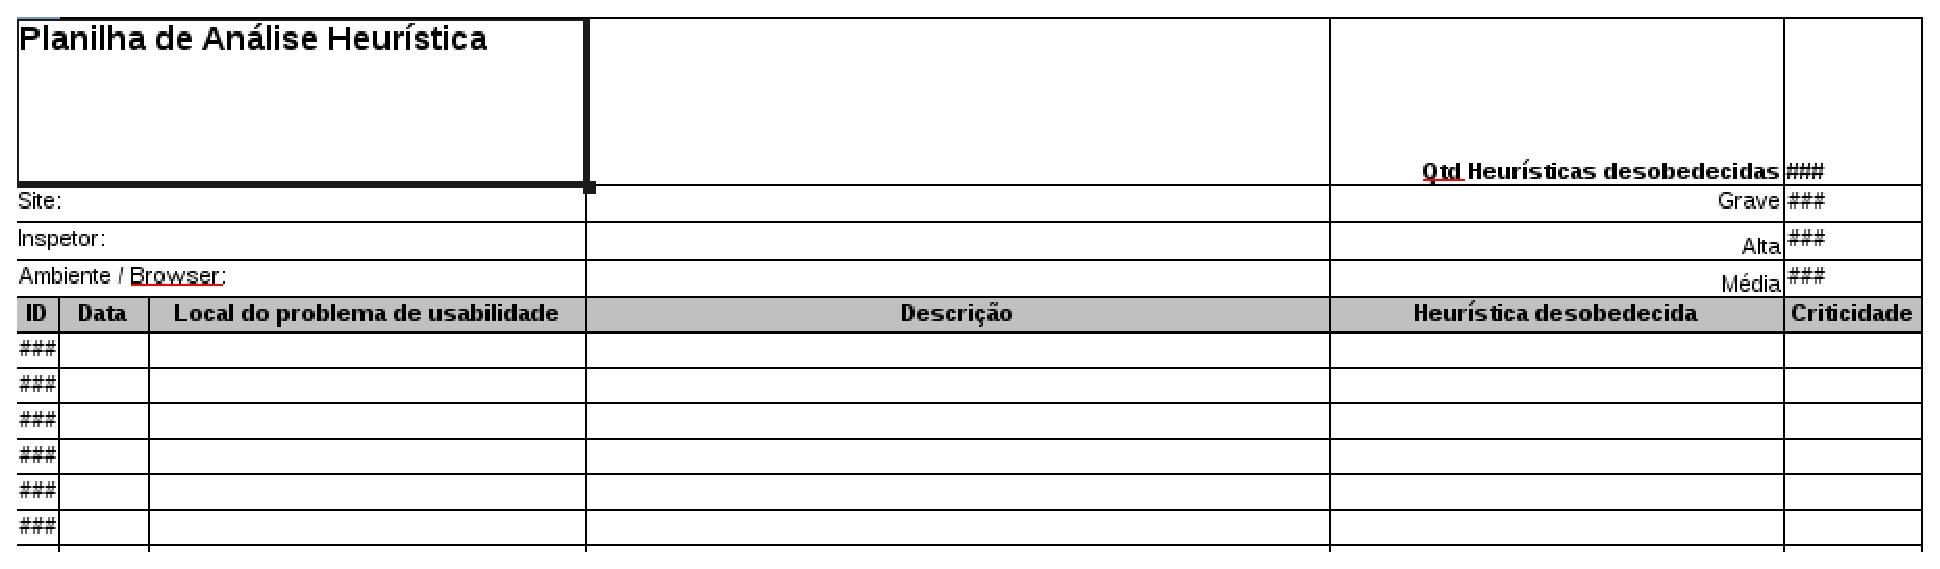
\includegraphics[keepaspectratio=true,scale=0.48]
      	{figuras/planilha.eps}
      	\label{planilha}
    	\caption{Planilha de Avaliação}
	\end{figure}

	A avaliação heurística requer pouco planejamento e pode fazer parte de um processo interativo de um projeto e aplicado em todas as fases de desenvolvimento da interface, mas é preciso conhecer as heurísticas para serem aplicadas.
\end{description}

%
No apêndice \ref{apendice1} estão detalhadas as técnicas mencionadas nesta seção.

%TODO isso foi inserido na introdução. Mas acho que talvez poderia criar uma seção, subseção sobre a usabilidade em software livre.
%TODO escrever outras coisas referente sobre software livre e usabilidade


%------------------------------------------------------------%
\section{Processos de Usabilidade}


	Alguns autores como ~\citeonline{mayhew1999} e ~\citeonline{hix1993} propuseram modelos de processo baseados em ciclo de vidas bem definidos para as atividades de usabilidade. O modelo estrela e o de Engenharia de Usabilidade propostos pelos autores estão definidos no \ref{apendice1}. 
	Outro modelo muito utilizado para descrever processos de usabilidade é o proposto pela norma ~\citeonline{iso:13407}, que define o Design Centrado no Usuário.

%TODO Uma parte foi inserido no apêndice (Modelo Estrela e o de Mayhew)

\subsection{Design Centrado no Usuário - DCU}

O DCU consiste em uma metodologia de \emph{design} de software. Definida pela norma ~\citeonline{iso:13407}, tem como objetivo definir um processo necessário ao desenvolvimento de produtos fáceis de utilizar na qual deve envolver os usuários no processo de desenvolvimento.

Sabemos que a ciência experimental que utiliza-se dos métodos empíricos tradicionais para coletar dados e testar hipóteses. Essa abordagem preocupa-se com os usuários quando as representa mas ela não leva em conta diversos aspectos do usuário real, por não envolvê-los no processo. Não basta fazer para o usuário, é preciso fazer com o usuário ~\cite{eason1995}. 

No DCU o usuário tem que ser o elemento central e é necessário envolvê-lo do início ao fim do projeto. Baseia-se nas necessidades, desejos e limitações das pessoas. ~\citeonline{travis2013} afirma que ``para criar produtos que os usuário amem, é necessário incluir os usuários no processo de criação dos produtos''. 


Existem quatro atividades de \emph{Design} Centrado no Usuário que devem estar presentes no inicío do projeto:

\begin{itemize}
\item Entender e especificar o contexto de uso;
\item Especificar os requisitos de usuário;
\item Produzir soluções de \emph{design};
\item Avaliar o \emph{design} frente aos requisitos;
\end{itemize}

A ~\citeonline{iso:13407} propõe que o envolvimento do usuário seja uma prática frequente em empresas que desenvolvem sistemas interativos.

\begin{figure}[h]
    \centering
    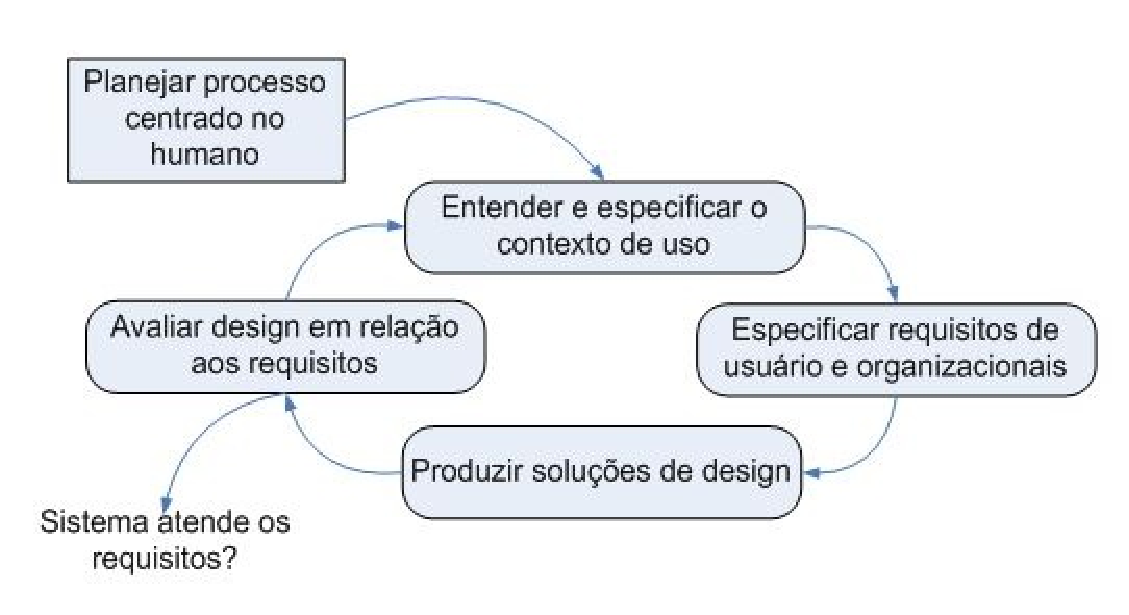
\includegraphics[keepaspectratio=true,scale=0.60]
      {figuras/ciclo_iso13407.eps}
    \caption{Ciclo do \emph{design} centrado no humano ~\cite{iso:13407}.}
    \label{ciclo_iso13407}
\end{figure}

\section{Aplicação de Usabilidade nos Métodos Empíricos}

	Partindo do que foi conceituado sobre desenvolvimento empírico e IHC, podemos ver semelhança entre seus valores, o que proporciona um quadro favorável à integração de práticas de usabilidade em desenvolvimento empírico. Podemos citar alguns desse valores: (i) ciclos curtos com entregas contínuas e incrementais, que favorecem a aplicação de técnicas de prototipagem; (ii) forte envolvimento do usuário que favorece a aplicação de princípios de projetos participativos e (iii) programação em pares onde em IHC geralmente a avaliação de usabilidade é feita em pares ~\cite{barbosa2008estrategia}. 
	%
	Segundo ~\citeonline{cybis2010} as características da abordagem ágil facilitam na utilização da ergonomia e da usabilidade durante o desenvolvimento de software.
		
	Porém adaptações são necessárias, principalmente na questão da granularidade da pesquisa, no tempo gasto com ela e na maneira de relatar as descobertas de usabilidade ~\cite{santos2012}.
	%
	~\citeonline{hodgetts2005experiences} afirma que os métodos de desenvolvimento empírico são quase sempre apresentados sob a visão dos programadores, deixando de lado outras disciplinas como Design de Experiência do Usuário. 
	
	No modo geral, os projetistas sabem da importância de desenvolver com enfoque no usuário e na usabilidade, mas normalmente os projetos são desenvolvidos sem que tenham sido realizadas pesquisas e aplicados métodos e técnicas de usabilidade.
%	
O tempo e os recursos limitados são as principais razões que impede a implantação dos testes de usabilidade nas equipes de desenvolvimento de software. Também há o desconhecimento por parte da equipe de desenvolvimento das técnicas a serem empregadas.
	
\begin{comment}
Alguns estudos foram feitos tentando fazer essa integração da usabilidade em desenvolvimento empírico.

~\citeonline{memmel2007} mostram que é possível unir IHC e engenharia de software sob a perspectiva ágil com a utilização de um ciclo de vida de interface de usuário multidisciplinar e de Engenharia de software chamado CRUISER.

Segundo ~\citeonline{mcinerney2005ucd} métodos ágeis e \emph{design} centrado no usuário possuem uma cultura distinta mas eles mostraram que é possível unir essas duas abordagens.

~\citeonline{lee2011} relata em seus estudos a utilização da abordagem de usabilidade ágil eXtreme Scenario-based \emph{design} (XSBD) na qual concluíram que os desafios que o time encontrava eram relacionados à comunicação, colaboração e compartilhamento de informação.

~\citeonline{wolkerstorfer2008probing} em seu estudo mostra adaptações feitas ao processo do XP. Ele integrou cinco instrumentos de IHC com o processo do XP. Os instrumentos são: testes de unidade estendidos para avaliação de usabilidade automatizada; Extreme Personas (variação do método clássico de personas); estudos de usuários para tomar conhecimento sobre o usuário final; avaliações feitas por especialistas em usabilidade e testes de usabilidade com usuários.
 
~\citeonline{leiteinspeccao}, analisou a utilização de métodos de inspeção da usabilidade no contexto de uma \textit{startup}. Foram abordados duas modalidades de avaliação heurística nessa pequena empresa de desenvolvimento de software que utiliza o método ágil Scrum. Como conclusão do estudo, relataram que a avaliação tradicional encontrou mais problemas de usabilidade e maior número de heurísticas violadas. Já na avaliação heurística colaborativa as médias de severidades atribuídas pelos avaliadores eram maior, no qual encontravam mais problemas sérios do que na avaliação tradicional, além de o tempo gasto foi menor do que na tradicional. A avaliação colaborativa apresentou características que permitia a melhor integração com ambientes ágeis.
\end{comment}

\subsection{Integração de práticas}
%\subsection{Integração de Práticas do IHC com o XP}

Alguns estudos foram encontrados tentando integrar práticas de usabilidade com os métodos empíricos. ~\citeonline{constantine2002process} foi um dos primeiros a iniciar a discussão sobre o tema. Sua proposta é mostrar que o DCU está prontamente integrado aos métodos ditos ``leves''. Ele afirma que XP e os demais métodos empíricos compartilham das mesmas fraquezas apresentadas por processos tradicionais como o processo unificado quando se refere à usabilidade e ao desenho de interface do usuário.

Em 2008 foi proposto uma metodologia revisional intitulada XPlus que insere as técnicas de \emph{design} e de usabilidade em determinadas fases do ciclo de desenvolvimento de software. O XPlus agrega algumas práticas de \textit{User Experience} às práticas tradicionais de XP. A figura \ref{ciclo_xplus} mostra o processo de desenvolvimento de software de XPlus ~\cite{guimaraesxplus}. 

O papel de \emph{designer} de interação não é reconhecido no núcleo XP da equipe e o XP não tem nenhum processo explícito para lidar com o \emph{design} de interação. 
%

\begin{figure}[h]
    \centering
    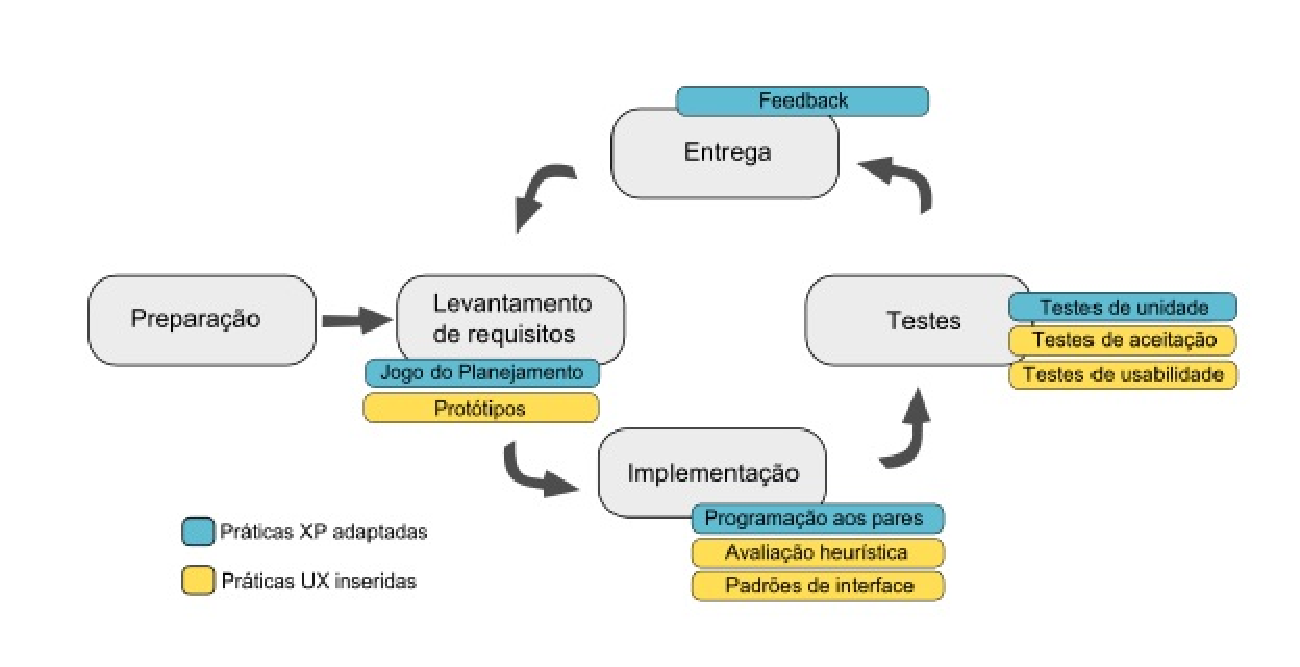
\includegraphics[keepaspectratio=true,scale=0.55]
      {figuras/xplus.eps}
    \caption{Visão geral do processo de desenvolvimento de software de XPlus ~\cite{guimaraesxplus}}
    \label{ciclo_xplus}
\end{figure}

O XPU, processo ágil centrado em usabilidade descrito por ~\citeonline{vasconcelos2003integrando} tinha como objetivo prover à equipe de desenvolvimento um modelo para a construção de sistemas de software centrado no usuário que valorizasse a usabilidade como característica fundamental da qualidade. 

O XPU serve para guiar o time de desenvolvimento seguindo técnicas e artefatos simplificados afim de não se ter apenas sistemas portáteis reutilizáveis ou acoplados, mas sim com uma interface que reflete as características e as necessidades dos usuários. 
%
%O método XPU foi definido a partir do processo de usabilidade Praxis-u (Padua, 2006). 
As atividades no XPu estão divididas em atividades técnicas e gerenciais. As atividades técnicas estão relacionadas à execução correta do processo de usabilidade, já as gerenciais garantem o controle e execução dessas práticas.

Nas próximas tabelas são apresentadas as atividades técnicas e gerenciais de cada visão (projeto, iteração e desenvolvimento) estabelecidas pelo XP e adaptadas pelo método XPu:

\begin{itemize}
\item {Visão de Projeto}
\begin{itemize}
\item {Atividades Técnicas}

\begin{table}[h]
\scalefont{.85}
\begin{tabular}{|p{4cm}|l|p{8cm}|}
\hline
\textbf{Atividade}                                                                       & \textbf{Técnica}                                                    & \textbf{Descrição}                                                                                                                                                                                  \\ \hline
Análise de Usuários                                                                      & Personas                                                            & Caracterizar grupos de usuários finais. Descrever expectativas de um usuário em relação ao desenvolvido.   \\ \hline
Análise de Tarefas                                                                       & Roteiros                                                            & Propõe uma narrativa textual para descrever a execução de uma tarefa pelo usuário.            \\ \hline
\begin{tabular}[c]{@{}l@{}}Análise de Contexto \\ de uso\end{tabular}                    & \begin{tabular}[c]{@{}l@{}}Histórias de \\usabilidade\end{tabular} & São formadas pelo Roteiro sendo realizada pela Persona.                                          \\ \hline
Definição de requisitos e metas de usabilidade & Benchmarks & Servem de balizadores para avaliar a usabilidade. São gerados a partir dos atributos de usabilidade \\ \hline
\begin{tabular}[c]{@{}l@{}}Avaliação da Usabilidade\end{tabular}                      & \begin{tabular}[c]{@{}l@{}}Cenários de Testes\end{tabular}        & São utilizados como insumos de avaliações de usabilidade. \\ \hline
\begin{tabular}[c]{@{}l@{}}Avaliação da Usabilidade\end{tabular}                      & \begin{tabular}[c]{@{}l@{}}Testes de Usabilidade\end{tabular}    & Estes testes podem ser feitos através de avaliações preditivas, experimentais.                                                                            \\ \hline
\end{tabular}
\caption{Atividades Técnicas de Visão de Projeto}
\label{visao_projeto}
\scalefont{1}
\end{table}

\newpage

\item{Atividades Gerenciais}

\begin{table}[h]
\scalefont{.85}
\centering
\begin{tabular}{|l|l|l|l|l|}
\hline
\textbf{Atividade}  & \textbf{Técnica}  & \textbf{Descrição}  & Insumos  & Saídas      \\ \hline
\begin{tabular}[c]{@{}l@{}}Planejamento \\ de usabilidade\end{tabular} & \begin{tabular}[c]{@{}l@{}}Planning \\ Poker\end{tabular} & \begin{tabular}[c]{@{}l@{}}Ocorre simultaneamente ao \\ planejamento da release. O \\ Projetista de interação contribui\\ com o seu parecer sobre\\ as estimativas de tamanho \\ das histórias de usabilidade.\end{tabular}  & \begin{tabular}[c]{@{}l@{}}Histórias de \\ usabilidade e\\ Planejamento\\ das avaliações\end{tabular} & \begin{tabular}[c]{@{}l@{}}Estimativas \\ de Recursos\\ (Tempo e\\ Custo)\end{tabular}             \\ \hline
\begin{tabular}[c]{@{}l@{}}Controle de \\ Usabilidade\end{tabular}     & Velocity                                                  & \begin{tabular}[c]{@{}l@{}}Acompanhamento das tarefas \\ relativas à usabilidade, \\comparando o esforço previsto\\ com o realizado.\end{tabular}                                                                                                    & \begin{tabular}[c]{@{}l@{}}Estimativas de\\ recursos\end{tabular}                                    & \begin{tabular}[c]{@{}l@{}}Refinamento \\ de estimativas \\ e Velocidade\\ do projeto\end{tabular} \\ \hline
\end{tabular}
\caption{Atividades Gerenciais de Visão de Projeto}
\scalefont{1}
\end{table}

\end{itemize}

\item{Visão de Iteração}

\begin{table}[h]
\scalefont{.85}
\begin{tabular}{|l|l|l|l|l|}
\hline
\textbf{Atividade}                                                           & \textbf{Técnica}                                           & \textbf{Descrição}                                                                                                                                                                                                     & Insumos                                                              & Saídas                                                                  \\ \hline
\begin{tabular}[c]{@{}l@{}}Definição de estilos\\ de interação.\end{tabular} & Template                                                   & \begin{tabular}[c]{@{}l@{}}São modelos estruturados \\ de interface que permite definir\\ um guia de estilo padrão. O \\ guia de estilo descreve\\ diretrizes e padrões para\\ o desenvolvimento de software.\end{tabular} & \begin{tabular}[c]{@{}l@{}}Requisitos de \\ Usabilidade\end{tabular} & \begin{tabular}[c]{@{}l@{}}Guia de\\ estilos\\ (Templates)\end{tabular} \\ \hline
Desenho de Interação                                                         & \begin{tabular}[c]{@{}l@{}}Interface \\ Final\end{tabular} & \begin{tabular}[c]{@{}l@{}}As interfaces geradas \\devem estar em conformidade \\com os templates definidos\\ pelo projeto.\end{tabular}                                                                                & Templates                                                            & \begin{tabular}[c]{@{}l@{}}Interfaces\\ finais\end{tabular}             \\ \hline
\end{tabular}
\caption{Atividades Técnicas de Visão de Interação}
\scalefont{1}
\end{table}

\item{Visão de Desenvolvimento}

\begin{table}[h]
\scalefont{.85}
\begin{tabular}{|l|l|l|l|l|}
\hline
\textbf{Atividade}                                                  & \textbf{Técnica}                                                                 & \textbf{Descrição}                                                                                                                                                                                                                               & Insumos                                                       & Saídas                                                           \\ \hline
\begin{tabular}[c]{@{}l@{}}Prototipação de\\ Interface\end{tabular} & \begin{tabular}[c]{@{}l@{}}Prototipação\\ Rápida\end{tabular}                    & \begin{tabular}[c]{@{}l@{}}É feita através de protótipos \\ de baixa fidelidade em papel. \\São feitos pelos projetistas\\ de interação e apresentados \\aos usuários com objetivo\\ de avaliá-los e discutir \\alternativas de desenhos.\end{tabular} & Templates                                                     & \begin{tabular}[c]{@{}l@{}}Protótipo\\ Simplificado\end{tabular} \\ \hline
\begin{tabular}[c]{@{}l@{}}Avaliação de\\ Usabilidade\end{tabular}  & \begin{tabular}[c]{@{}l@{}}Podem ser\\ utilizadas várias\\ técnicas\end{tabular} & \begin{tabular}[c]{@{}l@{}}Diversas avaliações podem \\ser utilizadas durante o \\ciclo de desenvolvimento.\end{tabular}                                                                                                                          & \begin{tabular}[c]{@{}l@{}}Cenários \\ de Testes\end{tabular} &                                                                  \\ \hline
\end{tabular}
\caption{Atividades Técnicas de Visão de Desenvolvimento}
\scalefont{1}
\end{table}

\end{itemize}

\newpage

\subsection{DCU Ágil}

Pode ser definido o DCU ágil como a prática de \emph{design} centrado no usuário quando conduzida dentro de uma metodologia ou filosofia de desenvolvimento ágil de software ~\cite{santos2012}. 
%
O ciclo de DCU ágil foi proposto por ~\citeonline{sy2007adapting} e integra tantos as atividades de DCU como as de desenvolvimento em um único ciclo, trabalhando nas mesmas características e garantindo que as investigações de usabilidade serão tratadas durante a interação.
%
Segundo \citeonline{najafi2008} o \emph{design} centrado no usuário pode ser incorporado no desenvolvimento empírico sem grandes impactos no processo. No método de desenvolvimento ágil scrum, uma funcionalidade é desenvolvida, testada e documentada em uma \textit{sprint} assim como no \emph{design} centrado no usuário. 
%	
Segundo ~\citeonline{santos2012} o grande desafio do DCU ágil é encontrar a melhor maneira de realizar as atividades de pesquisa do usuário, \emph{design} de versões que atendem às necessidades dos usuário, construção de versões interativas e realização de testes de usabilidade, dentro de um ambiente de desenvolvimento empírico, tendo a participação dos usuários típicos em todas as atividades.

\subsection{Princípios de Desenvolvimento Empírico Aplicados ao DCU}

	Alguns princípios do desenvolvimento empírico foram levantados pela comunidade envolvida em usabilidade para a aplicação no \emph{design} de sistemas centrado no usuário.

\begin{enumerate}

\item Compreender e identificar as necessidades reais dos usuários

O Objetivo dessa etapa é conhecer o usuário alvo. Deve-se projetar ferramentas que irão dar suporte aos objetivos e atividades das pessoas.

\item Focar na essência

O foco na essência ajuda a desenvolver soluções que atendem às reais necessidades dos usuários diminuindo os riscos de desenvolvimento de funcionalidades com pouco ou nenhum uso.


\item Iterar mais rápido

	É importante colocar o produto nas mãos dos usuários para se ter um \textit{feedback} o mais cedo possível. Quando a iteração é feita de forma rápida e começando cedo podemos identificar os problemas com antecedência o que diminui o tempo com retrabalho e evita que o produto não atenda aos usuários.
	

\item Criar \emph{designs} alternativos

	Deve-se pensar em criar várias soluções para um mesmo problema afim de que possa ter mais possibilidades de escolha. 


\item Prototipação em baixa resolução

Os protótipos de baixa resolução permite visualizar uma solução de forma mais rápida e concreta economizando tempo de \emph{design} e desenvolvimento. Esses protótipos ajudam a comunicar e entender ideias e serve para validar uma solução. 

	
\item Menos documentação, mais comunicação

	É essencial que tenha uma boa comunicação em todo o processo entre os desenvolvedores, \emph{designs} e \textit{stakeholders} envolvidos no projeto.

%\item Pesquisa e \emph{design} em paralelo ao desenvolvimento


\item Testes de usabilidades ágeis

	Os testes de usabilidade devem ser feitos em todos os ciclos do projeto.  Os resultados encontrados nos testes devem ser comunicados à equipe para que possa corrigir possíveis erros.

\item O fim não é o lançamento

	No fim de cada ciclo lança-se o mínimo adequado às necessidades reais dos usuários. Ao observar o uso real identificamos que existem novas formas para usar a ferramenta e podemos propor novas melhorias para o sistema. 
	
\end{enumerate}


\section{Considerações}

	A integração entre os processos de usabilidade e os métodos empíricos é esperada e possível. Tanto o desenvolvimento empírico como os processo de usabilidade tem em comum características que colocam o foco do desenvolvimento nas necessidade e anseios dos usuários finais, na interação entre os \textit{stakeholders} envolvidos e na qualidade final do produto a ser desenvolvido. 
	
	Os testes de usabilidade e testes de aceitação muitas vezes são confundidos. Testes de aceitação podem trazer as questões de usabilidade, mas não é o único método para ser utilizado em um projeto. Por ser feito tardiamente as mudanças baseadas em testes de aceitação são muito mais caras. Já os testes de usabilidade foram projetados para oferecer informações verdadeiras de desempenho desde o início do processo.  
%
O principal objetivo dos testes de aceitação é servir como uma verificação final de que a aplicação atendeu aos requisitos funcionais estabelecidos pelo cliente ~\cite{preece2007}.

No proximo capítulo, utilizamos no estudo de caso algumas técnicas de usabilidade que foram aplicadas juntamente com os testes de desenvolvimento empírico de software.





